\section{第九回 ラプラス変換}
%-----------------------------------------------------------------------

\subsection{目的}

ラプラス変換とは何かを学ぶ。ラプラス変換により、微分方程式の
初期値問題が簡単に解けることを理解する。
ラプラス逆変換の公式を複素積分により導けるようにする。

\subsection{解答}

\ans{28}{1}

フーリエ変換の場合と同様に部分積分を行う。ただし、積分が$x=0$からであるため、
$f(0)$などが出てくることに注意。

\begin{eqnarray}
  {\cal L}[f'(x)] &=& \int_0^\infty \diff x f'(x)\e^{-sx} \\
  &=& \left[ -f(x)\e^{-sx} \right]_0^{\infty}  +  s \int_0^\infty \diff x f(x) \e^{-sx}\\
  &=& s {\cal L}[f(x)] + f'(0)
\end{eqnarray}
高次の微分も同様。

\ans{28}{2}

ラプラス変換の定義から、
\begin{equation}
  {\cal L}[\e^{ax }f(x)] = \int_0^\infty \diff x f(x)\e^{-(s-a)x}
\end{equation}
$s-a = s'$と思えば、
\begin{eqnarray}
  {\cal L}[\e^{ax }f(x)] &=& \int_0^\infty \diff x f(x)\e^{-s'x}\\
  &=& \hat{f}(s')\\
  &=& \hat{f}(s-a)
\end{eqnarray}

\ans{28}{3}
\begin{eqnarray}
  {\cal L}[f*g(x)] &=&  \int_{0}^{\infty} \diff x \e^{-sx} \int_{0}^{x} \diff y f(x-y)g(y)
\end{eqnarray}
ここで、積分順序を入れ替える。
\begin{equation}
  \int_0^{\infty} \diff x \int_0^{x} \diff y = \int_0^{\infty} \diff y \int_y^{\infty} \diff x
\end{equation}
に注意すると、
\begin{eqnarray}
  {\cal L}[f*g(x)] &=&  \int_0^{\infty} \diff y \int_y^{\infty} \diff x  \e^{-sx} f(x-y)g(y) \\
  &=& \int_0^{\infty} \diff y g(y) \int_y^{\infty} \diff x  \e^{-sx} f(x-y) \\
  &=& \int_0^{\infty} \diff y g(y) \e^{-py} \int_y^{\infty} \diff x  \e^{-s(x-y)} f(x-y) \\
  &=& \int_0^{\infty} \diff y g(y) \e^{-py} \int_0^{\infty} \diff x'  \e^{-sx'} f(x') \\
  &=& {\cal L}[g] {\cal L}[f]
\end{eqnarray}
ただし、途中で$x-y = x'$とおくことで、二項目の積分を$y$に依存しないようにした。


\ans{29}{1}
ラプラス変換の定義から、
\begin{eqnarray}
  {\cal L}[1] &=& \int_0^{\infty} \e^{-sx} \diff x\\
  &=& \frac{1}{s}
\end{eqnarray}

\ans{29}{2}
\begin{eqnarray}
  {\cal L}[\delta(x)] &=& \int_0^{\infty} \diff x \delta(x) \e^{-sx}\\
  &=& 1
\end{eqnarray}

\ans{29}{3}
\begin{eqnarray}
  {\cal L}[x] &=& \int_0^{\infty}  x \e^{-sx} \diff x\\
  &=& \left[ \frac{x \e^{-sx}}{-s} \right]_0^{\infty} + \frac{1}{s} \int_0^{\infty} \e^{-sx} \diff x\\
  &=& \left[ -\frac{\e^{-sx}}{s^2} \right]_0^{\infty} \\
  &=& \frac{1}{s^2}
\end{eqnarray}

\ans{29}{2}
\begin{eqnarray}
  {\cal L}[\e^{\alpha x}] &=& \int_0^{\infty}  \e^{\alpha x} \e^{-sx} \diff x\\
  &=& \int_0^{\infty}  \e^{-(s-\alpha)x} \diff x\\
  &=& \left[ - \frac{\e^{-(s-\alpha)x}}{s-\alpha}  \right]_0^{\infty}\\
  &=& \frac{1}{s-\alpha}
\end{eqnarray}
ただし、$x \rightarrow \infty$で$\e^{-(s-\alpha)x} \rightarrow 0$で
あるために、${\mathrm Re} s > \alpha$でなくてはならない。

\ans{30}{1}
逆ラプラス変換の定義から、
\begin{equation}
  f(x) = \frac{1}{2 \pi i} \int_{a-i\infty}^{\alpha+i\infty} \diff s \frac{\e^{sx}}{s-\alpha}
\end{equation}
ここで、複素積分を用いるが、$\e^{sx}$があるため、$x$の正負によって
積分範囲を変える必要がある。
$x>0$の時は図$\ref{fig_laplace_int}$の左のように積分路$C$を取ることで、
ジョルダンの補題から円弧の部分の積分の寄与は$0$である。
また、積分路の中には$z=\alpha$が一位の極として含まれるので、
留数定理より
\begin{eqnarray}
  f(x) &=& \frac{1}{2 \pi i} \int_C \diff z \frac{\e^{zx}}{z-\alpha}\\
  &=& \e^{\alpha x}
\end{eqnarray}

$x<0$の場合は逆向きに積分路を取る。このとき、
積分路の中には極が含まれないため、
\begin{equation}
  f(x) = 0
\end{equation}
以上から、
\begin{equation}
  f(x) = \left\{
  \begin{array}{cc}
    0       & \qquad x<0 \\
    \e^{ax} & \qquad x>0
  \end{array}
  \right.
\end{equation}


\begin{figure}[htbp]
  \begin{center}
    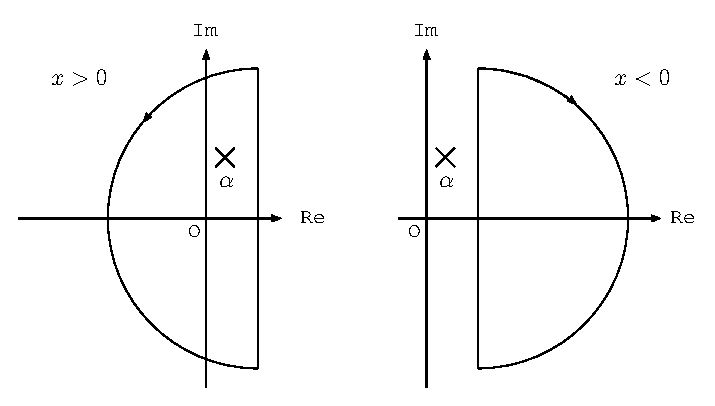
\includegraphics[width=.5\linewidth]{fig/laplace_int.eps}
  \end{center}
  \caption{
    ラプラス逆変換を行うための積分路。
    ジョルダンの補題により、$\e^{sx}$があるため、$x>0$の場合は
    左、$x<0$の場合は右を周る積分路を取らなくてはならない。
    このとき、ラプラス変換が存在する条件は、$s$の実部が
    すべての極の実部よりも大きいことなので、$x<0$の場合は
    必ず$0$となる。
  }
  \label{fig_laplace_int}
\end{figure}

\ans{30}{2}

前問と同様に$x<0$では$f(x) = 0$となるので、$x>0$の場合のみ考える。
\begin{eqnarray}
  f(x) &=& \frac{1}{2 \pi i} \int_C \diff z \frac{z \e^{zx}}{z^2+c^2}
\end{eqnarray}
ここで、特異点は$z = ic, -ic$の二つで、それぞれ一位の極である。
$z = ic$における留数は、
\begin{equation}
  \left. \frac{z \e^{zx}}{z+ic} \right|_{z = ic} = \frac{1}{2}\e^{icx}
\end{equation}
同様に$z = -ic$における留数は、
\begin{equation}
  \left. \frac{z \e^{zx}}{z-ic} \right|_{z = -ic} = \frac{1}{2}\e^{-icx}
\end{equation}
両方足せば、
\begin{equation}
  f(x) = \frac{\e^{icx}+\e^{-icx}}{2} = \cos cx
\end{equation}
を得る。

\ans{31}{1}
微分方程式全体をラプラス変換すると、$f(0)=f'(0)=0$より、
\begin{equation}
  (s^2 - 2s +1) \hat{y}(s) = \frac{1}{s^2}
\end{equation}
すなわち、
\begin{equation}
  \hat{y}(s) = \frac{1}{s^2 (s-1)^2}
\end{equation}
これを部分分数分解すると、
\begin{equation}
  \hat{y}(s) = \frac{-2}{s-1} + \frac{1}{(s-1)^2} + \frac{2}{s} + \frac{1}{s^2}
\end{equation}
ここで、それぞれ
\begin{eqnarray}
  {\cal L}[\e^x] &=& \frac{1}{s-1}\\
  {\cal L}[x\e^x] &=& \frac{1}{(s-1)^2}\\
  {\cal L}[1] &=& \frac{1}{s}\\
  {\cal L}[x] &=& \frac{1}{s^2}
\end{eqnarray}
であるから、
\begin{equation}
  f(x) = -2 \e^{x}+x\e^x+2+x
\end{equation}

微分方程式全体をラプラス変換すると、$f(0)=f'(0)=0$より、
\begin{equation}
  (s^2 + 2s +1) \hat{y}(s) = \frac{1}{s}
\end{equation}
すなわち、
\begin{equation}
  \hat{y}(s) = \frac{1}{s(s+1)^2}
\end{equation}
右辺を部分分数分解する。
やりかたを丁寧に解説すると、
\begin{equation}
  \frac{1}{s(s+1)^2} = \frac{a}{s} + \frac{b}{s+1} + \frac{c}{(s+1)^2}
\end{equation}
と分解できたとすると、両辺に$s$をかけてから$s=0$を代入すれば、
それは$a$である。
すなわち、
\begin{equation}
  a = \left. \frac{1}{(s+1)^2}\right|_{s=0} = 1
\end{equation}
同様に$(s+1)^2$を両辺にかけて$s=-1$を代入すれば、
\begin{equation}
  c = \left. \frac{1}{s}\right|_{s=-1} = -1
\end{equation}
$b$を求めるには、$(s+1)^2$を両辺にかけて微分してから$s=-1$を代入する。
よって、
\begin{equation}
  b = \left. \left(\frac{1}{s}\right)^2 \right|_{s=-1} = -1
\end{equation}
以上より、
\begin{equation}
  \hat{y}(s) =  \frac{1}{s} - \frac{1}{s+1} - \frac{1}{(s+1)^2}
\end{equation}
逆ラプラス変換すれば、
\begin{equation}
  y(x) =  1 - \e^{-x} - x\e^{-x}
\end{equation}
これは確かに$y(0)=y'(0) = 0$であり、
代入すると解になっている。


\subsection{解説}

\subsubsection{ラプラス変換}

フーリエ変換では、関数$f(x)$は無限区間$-\infty < x < \infty$で定義されていた。
変数を時間だと思えば、これは系に安定に存在する解について調べていることになる。
それに対し、電気回路にスイッチを入れたり、バネをはじいたりと、
それまで静的であった系になんらかの刺激を与えたときの応答を知りたい場合が
よくある。そのような過渡的な現象の解析に威力を発揮するのが
{\bf ラプラス変換 (Laplace transform)}である。
過渡的な現象は、微分方程式の初期値問題を解くことに帰着される。
ラプラス変換は、微分方程式の初期値問題を簡単に解く処方箋を与える。

\subsubsection{ラプラス変換とフーリエ変換}

ある関数$f(x)$に対して、次のような関数$g(x)$を考える。
\begin{equation}
  g(x) = \left\{
  \begin{array}{cc}
    0             & \qquad x<0      \\
    \e^{-ax} f(x) & \qquad x \geq 0
  \end{array}
  \right.
\end{equation}

ここで、$g(x)$をフーリエ変換すると、
\begin{eqnarray}
  {\cal F}[g(x)] &=& \int_{-\infty}^{\infty} \diff x g(x) \e^{-ikx}\\
  &=& \int_{0}^{\infty} \diff x \e^{-ax} f(x) \e^{-ikx}\\
  &=& \int_{0}^{\infty} \diff x f(x) \e^{-(a+ik)x}
\end{eqnarray}
ここで、$s = a+ik$とすると、
\begin{eqnarray}
  \int_{0}^{\infty} \diff x f(x) \e^{-(a+ik)x} &=& \int_{0}^{\infty} \diff x f(x) \e^{-sx}\\
  &=& {\cal L}[f(x)]
\end{eqnarray}
これは$f(x)$のラプラス変換に他ならない。
フーリエ変換不可能な関数でも、$a$を十分に大きく取れば$\e^{-ax} f(x)$の
積分が収束し、ラプラス変換が可能である場合がある。
すなわち、ラプラス変換とは、$\e^{-ax}$をかけて収束範囲を広げた
フーリエ変換と考えることができる。

さて、${\cal F}[g(x)]$をフーリエ逆変換しよう。
\begin{eqnarray}
  g(x) &=& \frac{1}{2\pi} \int_{-\infty}^{\infty} \diff k {\cal F}[g(x)] \e^{ikx}\\
  &=& \frac{1}{2\pi} \int_{-\infty}^{\infty} \diff k \hat{f}(s) \e^{ikx}
\end{eqnarray}
ここで、${\cal F}[g(x)] = \hat{f}(s)$であり、$x>0$であれば$g(x) = \e^{-ax} f(x)$であるから、
\begin{eqnarray}
  \e^{-ax} f(x) &=& \frac{1}{2\pi }  \int_{-\infty}^{\infty} \diff k \hat{f}(s) \e^{ikx}\\
  f(x) &=& \frac{1}{2\pi }  \int_{-\infty}^{\infty} \diff k \hat{f}(s) \e^{(a+ik)x}\\
\end{eqnarray}
$s = a + ik$と置くと、$\diff s = i \diff k$、
積分範囲が$a - \infty < s < a + \infty $となることから、
\begin{equation}
  f(x) = \frac{1}{2\pi i}  \int_{a-\infty}^{a+\infty} \diff s \hat{f}(s) \e^{sx}\\
\end{equation}
これは、ラプラス逆変換の定義である。

ここで$a$は 積分
\begin{equation}
  \int_0^{\infty} \e^{-ax} |f(x)| \diff x
\end{equation}
が収束するように選ばれたのであった。これは、$a$が$f(x)$のすべての極よりも
右側にくることを意味する\footnote{ここでは詳細は省略する。参考書を参照のこと}。
これによりラプラス逆変換が$x<0$の時に$f(x)=0$となる。
また、$s = a + ik$とおいたので、${\mathrm Re} s = a$である。
ラプラス変換において、$s$は一般に任意の複素数であるが、その実部は十分に
(ラプラス変換が収束するように)選ばれなければならない。

\subsubsection{非同次方程式とたたみ込み積分}

ラプラス変換は、線形非同次方程式を解くのに威力を発揮する(以下線形を略す)。
非同次方程式とは、次のような形の微分方程式である。
\begin{equation}
  u''(x) + u(x) = f(x) \label{eq_laplace_combo1}
\end{equation}

まず、$f(x)=\delta(x)$と置いた方程式を
\begin{equation}
  v''(x) + v(x) = \delta(x)
\end{equation}
と書こう。この解$v(x)$が得られたとすると、$u$を$v$で表すことができる。
まず、方程式全体をラプラス変換することで、
\begin{equation}
  {\cal L}[v] = \frac{1}{s^2+1} \label{eq_laplace_combo2}
\end{equation}
であることが分かる。
また、式(\ref{eq_laplace_combo1})をラプラス変換すれば、
\begin{equation}
  {\cal L}[u] = \frac{{\cal L}[f]}{s^2+1}\label{eq_laplace_combo3}
\end{equation}
である。式(\ref{eq_laplace_combo2})と式(\ref{eq_laplace_combo3})を見比べれば、
\begin{equation}
  {\cal L}[u] = {\cal L}[v] {\cal L}[f]
\end{equation}
たたみ込み積分のラプラス変換の性質から
${\cal L}[v] {\cal L}[f] = {\cal L}[v*f]$
であるから、
\begin{equation}
  u(x) = \int_0^{x} v(x-y)f(x)  \diff y
\end{equation}
と$u(x)$を$v(x)$で表すことができた。

すなわち、{\bf 同次方程式を解くことができれば、一般の
非同次方程式の解を得ることができる}。

デルタ関数とたたみ込み積分には物理的に重要な関係がある。
過渡的な現象にはたたみ込み積分が現れることが多い。
ある時刻$t=0$にデルタ関数的な刺激を与えたとき、
その出力(応答)が時刻$t$で$w(t)$となるような系を考える。
たとえば、LCR回路に瞬間的に電圧をかけたり、
ぴんと張った弦を弾いたりすると、系はしばらく振動して、
やがて落ち着いていくだろう。
このような応答を{\bf インパルス応答}と呼び、工学では特に重要な概念である。

デルタ関数に対する応答$w(t)$を用いて、任意の入力$f(x)$に対する
出力$h(t)$は
\begin{equation}
  h(t) = \int_0^t w(t-s) f(s) \diff s
\end{equation}
とたたみ込み積分の形で書くことができる。
この式は、時刻$s$での入力$f(s)$が、重み$w(t-s)$で
時刻$t$での出力$h(t)$に影響を与えているという意味を持っている。

%-----------------------------------------------------------------------
\section{おわりに}
%-----------------------------------------------------------------------

以上、物理で使われる数学を一通り学んだ。
かなり駆け足でやったので消化不良のところがあることだろう。
必要に応じて復習して欲しい。その際、教科書を読むだけでなく、
実際に手を動かしてみないと数学は身につかない。
物理で扱う方程式とその解には全て意味がある。
たとえば過渡的な現象であれば$t\rightarrow \infty$で$0$となるはずだろう。
波動方程式の解であれば、なんらかの波を表しているはずだから
周期的な運動を記述するだろう。
問題を解く際にはこのようなイメージを大事にして欲しい。

今回、電磁気学や流体力学で必要となるベクトル解析に
全く触れることができなかった。また、線形代数の扱いは不十分である。
必要であれば各自勉強して欲しい。

\end{document}


